
\documentclass[12pt,ngerman,parskip=full]{scrartcl}

\usepackage{babel}
\usepackage{blindtext}
\usepackage{tikz}

\begin{document}

\blindtext

\begin{center}
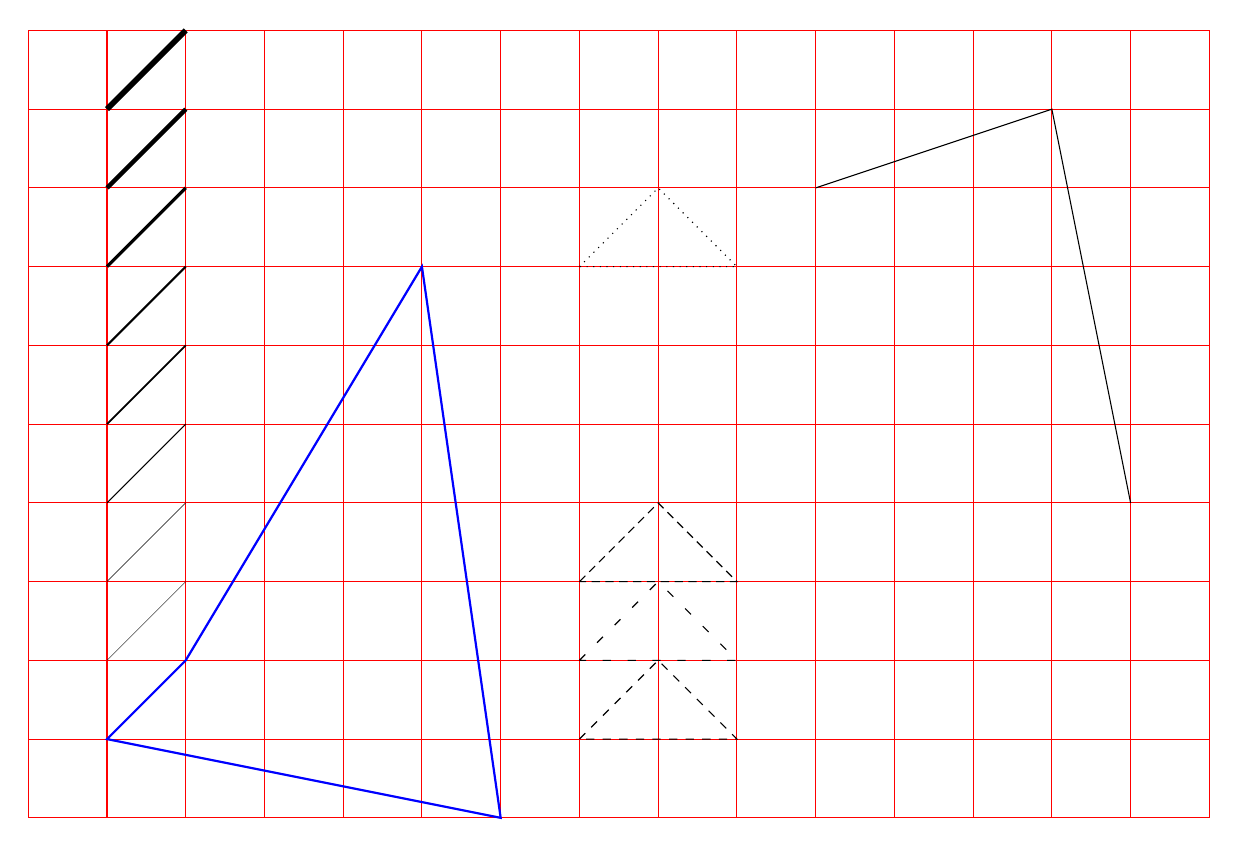
\begin{tikzpicture}
\draw[step=1cm,red,thin] (0,0) grid (15,10);
\draw[ultra thin] (1,2) -- (2,3);
\draw[very thin] (1,3) -- (2,4);
\draw[thin] (1,4) -- (2,5);
\draw[semithick] (1,5) -- (2,6);
\draw[thick] (1,6) -- (2,7);
\draw[very thick] (1,7) -- (2,8);
\draw[ultra thick] (1,8) -- (2,9);
\draw[line width = 2pt] (1,9) -- (2,10);

\draw[thick, blue] (1,1) -- (2,2) -- (5,7) -- (6,0) -- cycle ;

\draw[dotted] (7,7) -- (8,8) -- (9,7) -- cycle;

\draw[densely dashed] (7,3) -- (8,4) -- (9,3) -- cycle;
\draw[loosely dashed] (7,2) -- (8,3) -- (9,2) -- cycle;
\draw[dashed] (7,1) -- (8,2) -- (9,1) -- cycle;

\draw (10,8) -- ++(3,1) -- ++(1,-5);
\end{tikzpicture}
\end{center}

\blindtext


\end{document}